\documentclass[12pt]{article}
\usepackage{MinionPro}
\usepackage{CJK}
%\usepackage[scaled=0.85]{beramono}  %%% scaled=0.775
\usepackage[T1]{fontenc}
\usepackage{graphicx,booktabs,tabularx,psfrag}
\usepackage{xcolor}
\usepackage[a4paper]{geometry}
\usepackage{url}

\usepackage{pstool}

\usepackage{graphicx}
\begin{document}
\begin{CJK}{UTF8}{cwmb}
\renewcommand{\figurename}{圖}

\voffset=-1cm
\textwidth=5.6in
\textheight=9.2in

\newenvironment{num}
 {\leftmargini=6mm\leftmarginii=8mm
  \begin{enumerate}\itemsep=-2pt}
 {\end{enumerate}}

\newenvironment{sol}
 {\begin{quote}\mbox{}\llap{\color{blue}{解答:}\rule{10mm}{0pt}}\hspace*{-4pt}}{\end{quote}}


\thispagestyle{empty}
\fontsize{12}{20pt}\selectfont
\begin{center}
{\large\CJKfamily{cwyb}{經濟學原理下, 習題9}}\\[3mm]
劉彥佑 (R99628130)\\
李卿澄 (B97501046)\\
黃博億 (B99101014)\\
王祉婷 (B00704056)
\end{center}

\begin{num}
\item 
	\begin{num}
		\item 美國利率升高,代表美元存款能有較高的報酬,美元資產的投資報酬率也可能會跟著升高。相對於亞洲股市如果未來不看好的話,國際資金會選擇報酬率較高的美元資產,因此國際上的投資資金撤離亞洲股市,兌換成美元。
		\item 圖1以日圓為例,國際資金撤離日本使日圓需求減少,日圓貶值。
		\begin{figure}[htp]
			\centering
			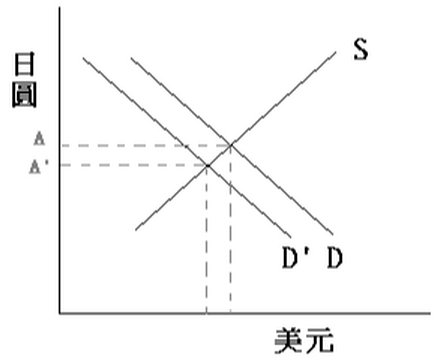
\includegraphics[scale=0.30]{jpus.png}
			\caption{日圓美元間之供給需求}
			\label{}
		\end{figure}
	\end{num}
\item 
	\begin{num}
		\item 2011年12月時,新台幣匯率為166.08元,而韓元匯率為168.02,新台幣相對韓元升值。
		\begin{figure}[htp]
			\centering
			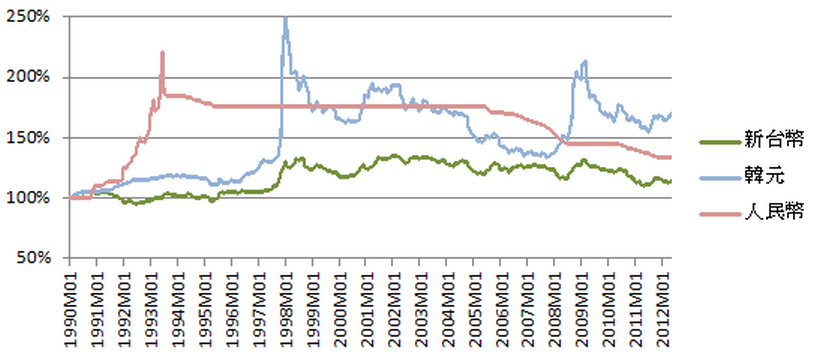
\includegraphics[scale=0.4]{tkr.png}
			\caption{新台幣與韓元對美元匯率}
			\label{}
		\end{figure}
		\item 2011年12月時,新台幣對韓元匯率為96.74,新台幣相對韓元升值。
		\begin{figure}[htp]
			\centering
			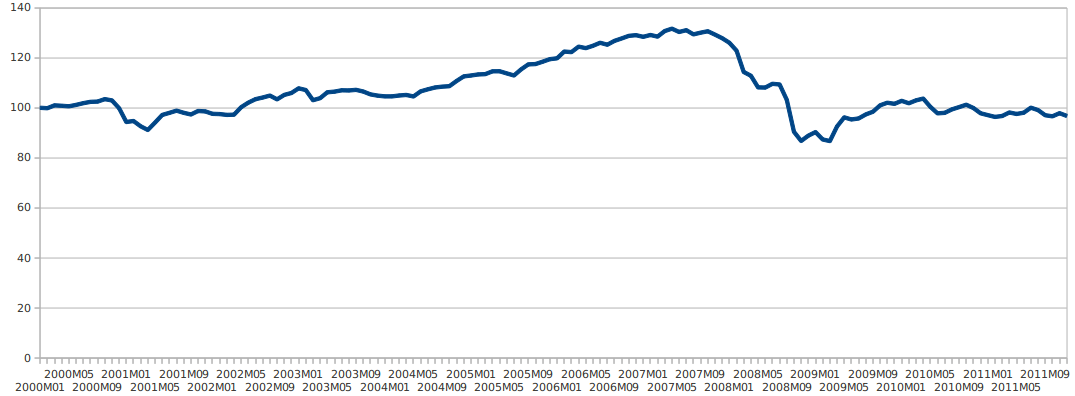
\includegraphics[scale=0.4]{ntdk.png}
			\caption{新台幣對韓元匯率}
			\label{}
		\end{figure}
		\item 2004~2007年間,新台幣對於韓元呈現貶值走勢,對於出口廠商有利,此時張忠謀董事長應該不會有穩定對韓元匯率的訴求。如果在2004年~2007年間,央行使台幣升值以穩定對韓元的匯率,那麼台積電的收入(兌換成台幣的部分)會減少,台積電的董事長如果此時提出穩定對韓元匯率的訴求,會遭到股東的反彈。
		\item 關於此篇投書的說法,我們認為如果新台幣在短期內因為熱錢的大量匯入,而造成大幅度的升值,我贊成央行應該要穩定匯率,減少對出口廠商的衝擊。因為台灣的中小企業占了很高的比例,如果每家廠商都對於匯率上的避險花費很大的心力,那麼總體而言會付出很大的成本。
		\\但是如果台幣的升值是長期的趨勢,而且央行不干預情況下的市場均衡價格與央行干預價格差一大截的話(例如課本247頁的例子:1985~1988年緩慢升值),那麼央行等於是買貴了美金,造成國家財富的損失。
	\end{num}
\end{num}
\end{CJK}
\end{document}
